\documentclass[tikz]{standalone}

% tikz
\usepackage{tikz, pgfplots}
\usepackage{prerex}
% i wish external worked but idk it sucks
%\usetikzlibrary{external}
%\tikzexternalize[prefix=figures/]

% for function graph
\usetikzlibrary{positioning}
\usetikzlibrary{shapes.geometric}
\usetikzlibrary{positioning}
\usetikzlibrary{shapes.misc}
\tikzset{
dot/.style = {circle, fill=#1, minimum size=5pt,
              inner sep=0pt, outer sep=0pt},
dot/.default = black % size of the circle diameter
}
\tikzset{cross/.style={cross out, draw=black, minimum size=2*(#1-\pgflinewidth), inner sep=0pt, outer sep=0pt},
%default radius will be 1pt. 
cross/.default={1pt}}

 % for braces
\usetikzlibrary{decorations.pathreplacing}
% for hashing area
\usetikzlibrary{patterns}
% tableaux var, signe
% source https://www.sqlpac.com/fr/documents/latex-package-tkz-tab-tikz-tableaux-de-signes-et-de-variations-de-fonctions.html
\usepackage{tkz-tab}
\input{../../colors}
\input{../../letterfonts}


\tikzset{
	every node/.style = {font=\Large}
}

\tikzset{
	every axis/.style = {clip=true, grid style = {opacity=.5}}
}
\tikzset{
	every node/.style = {font=\normalsize}
}

\begin{document}
%
	% page 1
	% 1-fonctions.tex
	% exe:graph-droite
	\begin{tikzpicture}[>=stealth]
		\begin{axis}[xmin = -5.5, xmax=3.5, ymin=-3.5, ymax=7.5, axis x line=middle, axis y line=middle, axis line style=->, grid=both]
			\addplot[no marks, BLUE_E, very thick, -] expression[domain=-5:3, samples=2]{1-x} 
			node[above, pos=.4] {$\Ccal_f$};
		\end{axis}
	\end{tikzpicture}
	
	% page 2
	% 1-fonctions.tex
	% exe:f-equals-g
	\begin{tikzpicture}[>=stealth]
		\begin{axis}[xmin = -2.5, xmax=2.3, ymin=-4.1, ymax=4.6, axis x line=middle, axis y line=middle, axis line style=->, grid=both,
			grid style = {opacity=.5},
			x=1.5cm,
			xtick={-3, -2, ..., 2},
			y=25pt,
			clip=true,
			]
			\addplot[no marks, BLUE_E, -, very thick] expression[domain=-2.5:2.3, samples=101]{(x-1)*(x-2)*(x+2)/2}
			node[pos=.5, above]{$\mathcal{C}_f$};
			\addplot[no marks, RED_E, -,  very thick] expression[domain=-2.5:2.3, samples=101]{1/(x-2.4) + 1/(x+2.6) + 2*x}
			node[pos=.65, above]{$\mathcal{C}_g$};
		\end{axis}
	\end{tikzpicture}
	
	% page 3
	% 1-fonctions.tex
	% exe:proj-xp1
	\begin{tikzpicture}[>=stealth]
		\begin{axis}[xmin = 0, xmax=4, ymin=0, ymax=5, axis x line=middle, axis y line=middle, axis line style=->, grid=both, x=50pt, y=50pt, extra x ticks ={0}, extra y ticks = {0}, ytick distance=1,]
			\addplot[no marks, BLUE_E, very thick, -] expression[domain=0:4, samples=2]{x+1} 
			node[above left, pos=.8] {$\Ccal_f$};
			\addplot[RED_E, mark=*, mark size = 2] (2,1) node[right] {$A$};
			\addplot[GREEN_E, mark=*, mark size = 2] (1,2) node[left] {$B$};
		\end{axis}
	\end{tikzpicture}
	
	
	% page 4
	% 1-equations.tex
	% exe:calendrier
    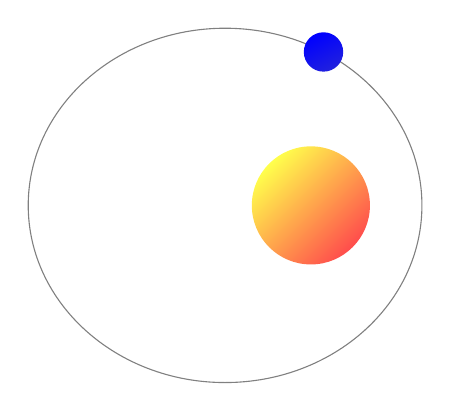
\begin{tikzpicture}[scale=2.5]
        \def\rS{0.3}                                % Sun radius

        \def\rE{0.1}                                % Earth radius
                                                    % Major radius of Earth's elliptical orbit = 1
        \def\eE{.9}                               % Excentricity of Earth's elliptical orbit       
        \pgfmathsetmacro\bE{.9}        % Minor radius of Earth's elliptical orbit  
          
        % This function computes the direction in which light hits the Earth.
        \pgfmathdeclarefunction{f}{1}{%
            \pgfmathparse{
                ((-\eE+cos(#1))<0) * ( 180 + atan( \bE*sin(#1)/(-\eE+cos(#1)) ) ) 
                +
                ((-\eE+cos(#1))>=0) * ( atan( \bE*sin(#1)/(-\eE+cos(#1)) ) ) 
            }
        }

        % This function computes the distance between Earth and the Sun,
        % which is used to calculate the varying radiation intensity on Earth.
        \pgfmathdeclarefunction{d}{1}{%
            \pgfmathparse{ sqrt((-\eE+cos(#1))*(-\eE+cos(#1))+\bE*sin(#1)*\bE*sin(#1)) }
        }

        % Draw the elliptical path of the Earth.
        \draw[thin,color=gray] (0,0) ellipse (1 and \bE);

        % Draw the Sun at the right-hand-side focus
        \shade[
            top color=yellow!70,
            bottom color=red!70,
            shading angle={45},
            ] ({sqrt(1-\bE*\bE)},0) circle (\rS);
         %\draw ({sqrt(1-\b*\b)},-\rS) node[below] {Sun};

        % Produces a series of frames showing one revolution
        % (the total number of frames is controlled by macro \N)
        \pgfmathtruncatemacro{\N}{12}
        \foreach \k in {2}{
            \pgfmathsetmacro{\Earthangle}{360*\k/\N}
            \pgfmathsetmacro{\Moonangle}{3*360*\k/\N} % <--- change the multiplying factor to suit your needs
            % Draw the Earth at \Earthangle
            \pgfmathsetmacro{\radiation}{100*(1-\eE)/(d(\Earthangle)*d(\Earthangle))}
            \colorlet{Earthlight}{yellow!\radiation!blue}
            \pgfmathparse{int(\k+1)}
                \shade[
                    top color=Earthlight,
                    bottom color=blue,
                    shading angle={90+f(\Earthangle)},
                    ] ({cos(\Earthangle)},{\bE*sin(\Earthangle)}) circle (\rE);
                 %\draw ({cos(\Earthangle)},{\bE*sin(\Earthangle)-\rE}) node[below] {Earth};  

        }
    \end{tikzpicture}
%
\end{document}